\begin{frame}
    \frametitle{In Progress Stage 1-4: FHR Benchmark Phase III Goals}
    \begin{itemize}
        \item FHR Benchmark Phase III: 3D full core with feedback and multicycle 
        analysis
        \item I will use the open-source MSR simulation tool, Moltres, to conduct
        AHTR multiphysics simulations for fuel slab and $\frac{1}{3}$
        fuel assembly geometries 
        \item AHTR Moltres simulations will capture thermal feedback effects, 
        absent from the purely neutronics OpenMC simulations
    \end{itemize}
\end{frame}

\begin{frame}
    \frametitle{In Progress Stage 1-4: Benchmark Phase III Preliminary Work}
    For successful AHTR Moltres simulation, I must establish 
    suitable spatial and energy homogenization that preserves accuracy while 
    maintaining an acceptable runtime
\begin{block}{Spatial Homogenization}
    Fuel slab discretization into 13 cells: FLiBe, left graphite, right graphite, 
    and ten fuel cells (each cell has a different packing fraction)
\end{block}
\begin{figure}[]
    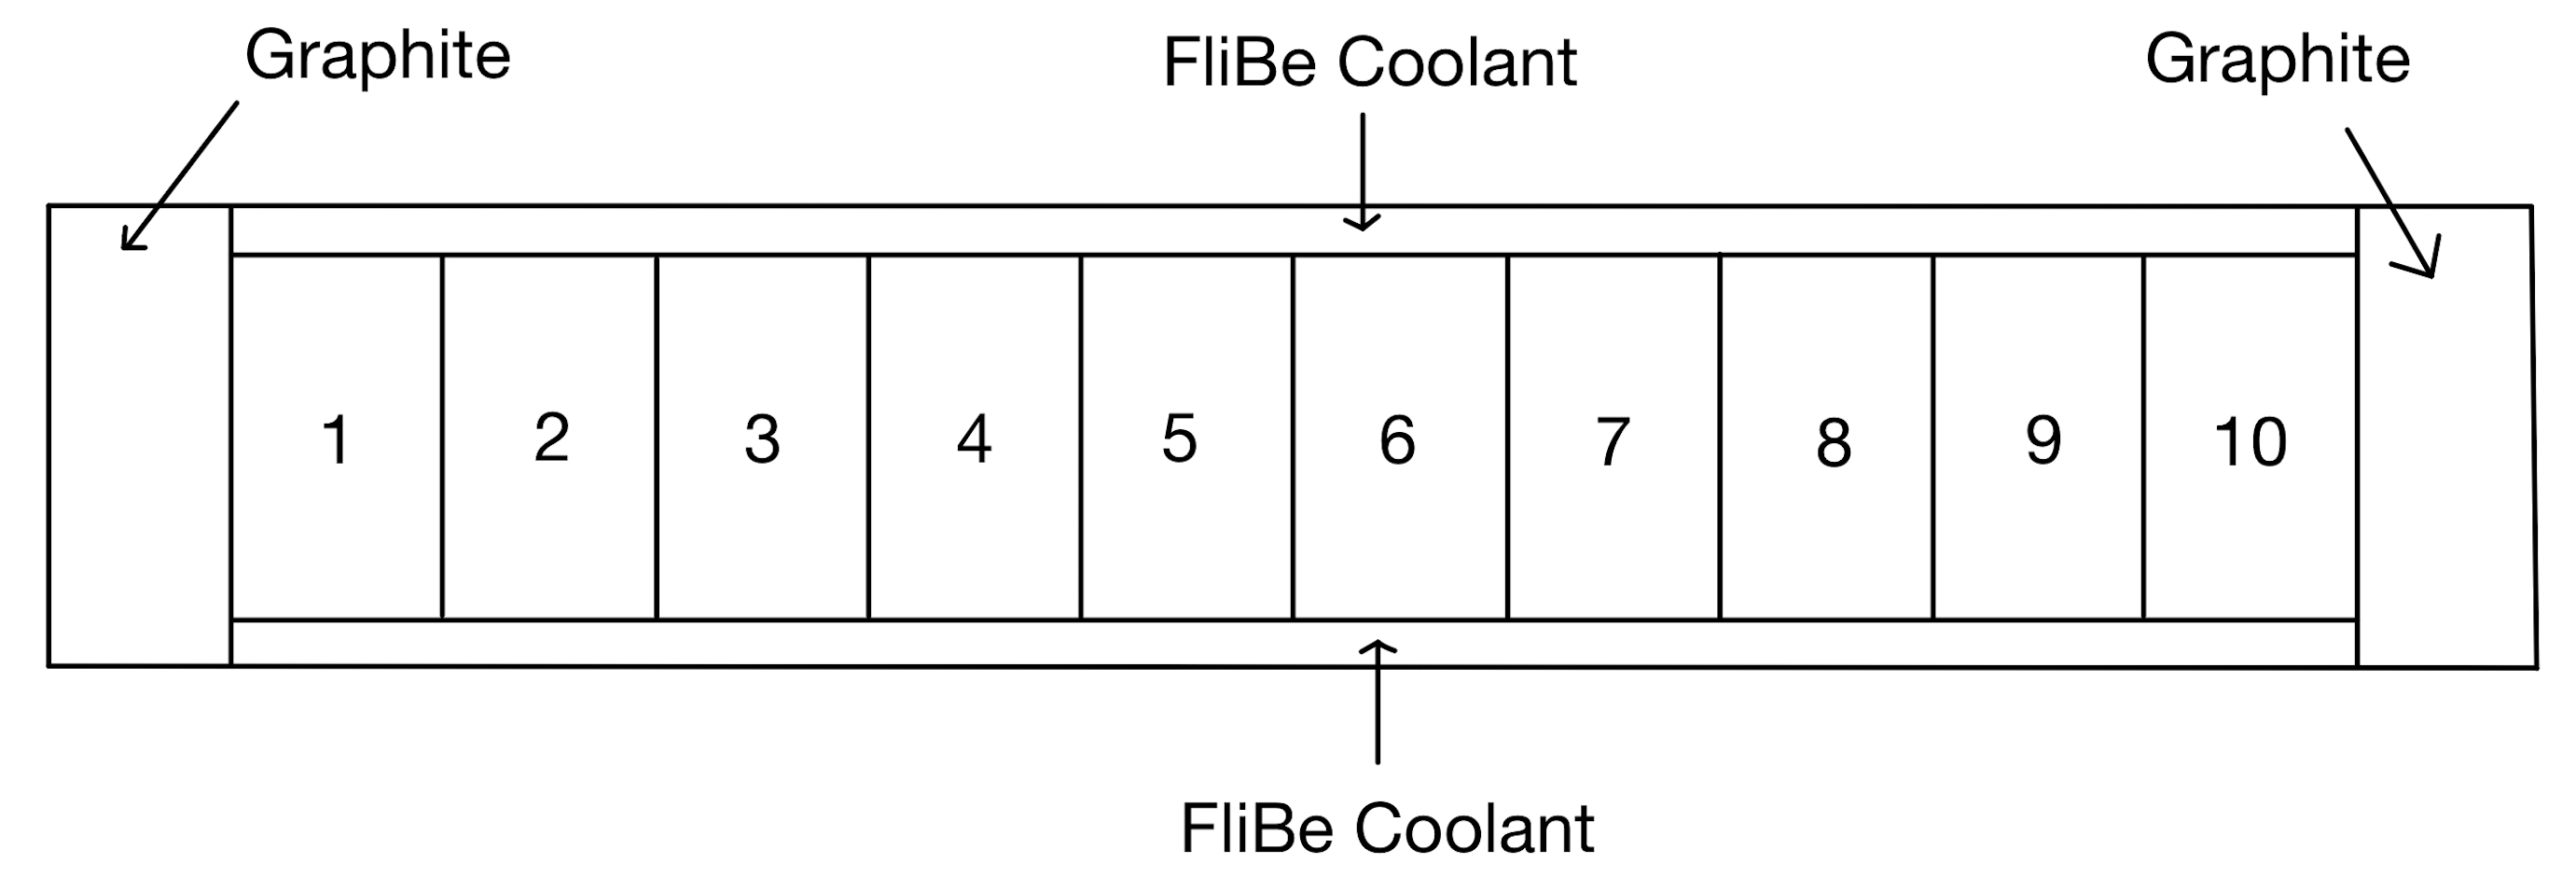
\includegraphics[width=0.8\linewidth]{figures/straightened_slab_mg.png}
    \caption{Straightened AHTR fuel slab spatially discretized into 
    13 \textit{cells} for OpenMC multigroup calculation.}
\end{figure}
\end{frame}

\begin{frame}
    \frametitle{In Progress Stage 1-4: Benchmark Phase III Preliminary Work}
    \begin{block}{Energy Homogenization}
        \begin{table}[]
            \centering
            \begin{minipage}[c]{0.6\textwidth}
                \centering
                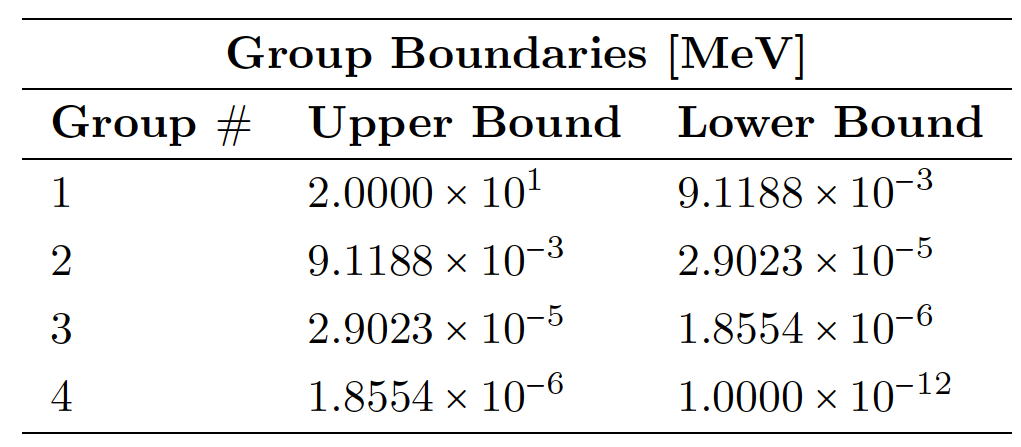
\includegraphics[width=0.9\linewidth]{figures/ahtr-energy-discr.png}
            \end{minipage}\hfill
            \begin{minipage}[c]{0.4\textwidth}
            \caption{4-group energy structures for AHTR geometry 
            derived by \cite{gentry_development_2016}.}
        \end{minipage}
        \end{table}
    \end{block}
    \vspace{-0.3cm}
    \begin{block}{Simulation Comparison: Continuous energy vs spatial 
        and energy homogenized}
        \begin{table}[]
                \centering
                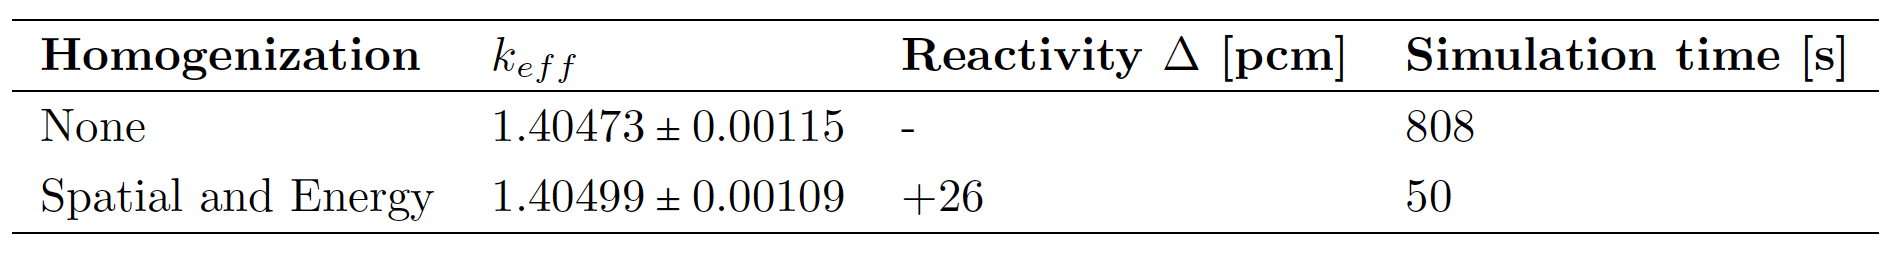
\includegraphics[width=0.9\linewidth]{figures/ahtr-homogenization.png}
            \caption{
                AHTR fuel slab's $k_{eff}$ for case with continuous energy and 
                space and case with spatial and energy homogenization.}
        \end{table}
    \end{block}
\end{frame}

\begin{frame}
    \frametitle{In Progress Stage 1-4: Benchmark Phase III Planned Work}
    \begin{itemize}
        \item Use these spatial and energy homogenization to set up a 
        Moltres AHTR plank steady-state simulation 
        \item Verify the Moltres model's neutronics parameters then run 
        the steady state simulation to determine maximum temperature 
        \item Test out energy and spatial homogenization methods for $\frac{1}{3}$
        fuel assembly Moltres model 
    \end{itemize}
\end{frame}